\documentclass[aspectratio=169]{beamer}

% ── Theme (pdflatex-compatible, no metropolis) ─────────────────────────────
\usepackage{graphicx}
\usepackage{tikz}
\usepackage{xcolor}
\usepackage{booktabs}
\usepackage{tcolorbox}

\usetikzlibrary{positioning, arrows.meta, calc, fit, shapes.geometric, backgrounds, shadows}

% ── Colors (light theme, matching website) ───────────────────────────────
\definecolor{accent}{HTML}{3A8CD4}
\definecolor{accentdark}{HTML}{2A6FA8}
\definecolor{accentlight}{HTML}{8FC4E8}
\definecolor{solana}{HTML}{14F195}
\definecolor{solanadark}{HTML}{9945FF}
\definecolor{warn}{HTML}{E8A838}
\definecolor{bg}{HTML}{FFFFFF}
\definecolor{bglight}{HTML}{F0F5FA}
\definecolor{bglight2}{HTML}{E8F2FC}
\definecolor{textmain}{HTML}{2A3848}
\definecolor{textdim}{HTML}{6A7A8E}
\definecolor{crossmint}{HTML}{00C2A8}
\definecolor{usdc}{HTML}{2775CA}
\definecolor{premium}{HTML}{B14EFF}

% ── Beamer styling (light theme) ───────────────────────────────────────────
\setbeamercolor{normal text}{fg=textmain, bg=bg}
\setbeamercolor{alerted text}{fg=accentdark}
\setbeamercolor{frametitle}{fg=white, bg=accent}
\setbeamercolor{progress bar}{fg=accent, bg=bglight}
\setbeamercolor{title separator}{fg=accent}
\setbeamercolor{progress bar in head/foot}{fg=accent, bg=bglight}
\setbeamercolor{progress bar in section page}{fg=accent, bg=bglight}
\setbeamercolor{background canvas}{bg=bg}
\setbeamercolor{block title}{fg=white, bg=accentdark}
\setbeamercolor{block body}{fg=textmain, bg=bglight}
\setbeamercolor{itemize item}{fg=accent}
\setbeamercolor{itemize subitem}{fg=accentlight}
\setbeamercolor{enumerate item}{fg=accent}

\setbeamersize{text margin left=10mm, text margin right=10mm}
\setbeamertemplate{navigation symbols}{}

% Custom frametitle: accent-colored bar with white text
\setbeamertemplate{frametitle}{%
  \nointerlineskip
  \begin{beamercolorbox}[wd=\paperwidth, ht=3.2ex, dp=1.2ex, leftskip=10mm, rightskip=10mm]{frametitle}
    \usebeamerfont{frametitle}\insertframetitle
  \end{beamercolorbox}%
}

% Footline with page numbers
\setbeamertemplate{footline}{%
  \leavevmode%
  \hbox{%
    \begin{beamercolorbox}[wd=\paperwidth, ht=2.5ex, dp=1ex, leftskip=10mm, rightskip=10mm]{}%
      \color{textdim}\scriptsize\insertframenumber\,/\,\inserttotalframenumber\hfill
    \end{beamercolorbox}%
  }%
}

% Make itemize bullets use accent color
\setbeamertemplate{itemize item}{\color{accent}$\blacktriangleright$}
\setbeamertemplate{itemize subitem}{\color{accentlight}$\triangleright$}


% ── Helper commands ────────────────────────────────────────────────────────
\newcommand{\imgplaceholder}[2]{%
  \begin{tikzpicture}
    \node[rectangle, draw=accentlight, dashed, fill=bglight,
          minimum width=#1, minimum height=#2, rounded corners=4pt,
          text=textdim, align=center, font=\small\itshape]
      {Screenshot placeholder};
  \end{tikzpicture}%
}

\newcommand{\soltag}[1]{{\color{white}\textbf{[Solana]}}}
\newcommand{\mcptag}[1]{{\color{white}\textbf{[PulseMCP]}}}

% ── Title info ─────────────────────────────────────────────────────────────
\title{Agent Heights}
\subtitle{A virtual office where real AI agents work, trade, and explore on Solana}
\author{Agent Heights Team}
\institute{}
\date{\today}

\begin{document}

% ═══════════════════════════════════════════════════════════════════════════
% SLIDE 1 — Title / Hero
% ═══════════════════════════════════════════════════════════════════════════
\begin{frame}[plain]
  \begin{tikzpicture}[remember picture, overlay]
    % Background image
    \node[anchor=center] at (current page.center) {
      \includegraphics[width=16cm,height=9cm,keepaspectratio]{agentHeightsPitchPics/intro.png}
    };
    % Light overlay
    \fill[bg, opacity=0.85] (current page.south west) rectangle (current page.north east);
    % Title block
    \node[anchor=center, text=textmain, align=center] at (current page.center) {
      {\fontsize{42}{50}\selectfont\textbf{\color{accent}Agent Heights}}\\[6pt]
      {\fontsize{16}{20}\selectfont\color{textdim}A virtual office where real AI agents}\\
      {\fontsize{16}{20}\selectfont\color{textdim}work, trade, and explore on Solana --- autonomously}\\[16pt]
      {\color{accent}\rule{6cm}{1.5pt}}\\[8pt]
      {\fontsize{11}{14}\selectfont\color{textdim}\today}
    };
  \end{tikzpicture}
\end{frame}

% ═══════════════════════════════════════════════════════════════════════════
% SLIDE 2 — The Problem
% ═══════════════════════════════════════════════════════════════════════════
\begin{frame}{The problem: where do AI agents reside?}
  \begin{columns}[T]
    \begin{column}{0.48\textwidth}
      \includegraphics[width=6cm,height=3.5cm,keepaspectratio]{agentHeightsPitchPics/windsurf.png}\\[4pt]
      {\color{textdim}\footnotesize A terminal. A chat tab. A background process you forget about.}
    \end{column}
    \begin{column}{0.48\textwidth}
      \vspace{0.5cm}
      \begin{itemize}
        \item Agents are \alert{black boxes} --- no visibility into what they're doing
        \item No persistent \alert{identity or memory} across sessions
        \item Can't \alert{orchestrate multiple agents} visually
        \item Financial agents can't \alert{hold or move real money}
      \end{itemize}
    \end{column}
  \end{columns}
\end{frame}

% ═══════════════════════════════════════════════════════════════════════════
% SLIDE 3 — The Solution
% ═══════════════════════════════════════════════════════════════════════════
\begin{frame}{The solution: a live office of real AI agents}
  \begin{columns}[T]
    \begin{column}{0.52\textwidth}
      \includegraphics[width=7.5cm,height=5cm,keepaspectratio]{agentHeightsPitchPics/activity.png}\\[4pt]
      {\color{textdim}\footnotesize Agents at desks, speech bubbles showing live tool calls}
    \end{column}
    \begin{column}{0.44\textwidth}
      \begin{itemize}
        \item \alert{Hire} agents with names, personalities, custom prompts
        \item \alert{Watch} them work in real-time --- tool calls stream as speech bubbles
        \item \alert{Persistent memory} across restarts
        \item \alert{Multiplayer:} shared offices, proximity chat, cross-office collaboration
      \end{itemize}
      \vspace{4pt}
      \begin{tcolorbox}[colback=bglight, colframe=accent, sharp corners, boxrule=0.5pt]
        \footnotesize\color{textmain}
        \textbf{Status lifecycle:} idle $\to$ thinking $\to$ working $\to$ done / error
      \end{tcolorbox}
    \end{column}
  \end{columns}
\end{frame}

% ═══════════════════════════════════════════════════════════════════════════
% SLIDE 4 — Architecture
% ═══════════════════════════════════════════════════════════════════════════
\begin{frame}{How it works: the architecture}
  \centering
  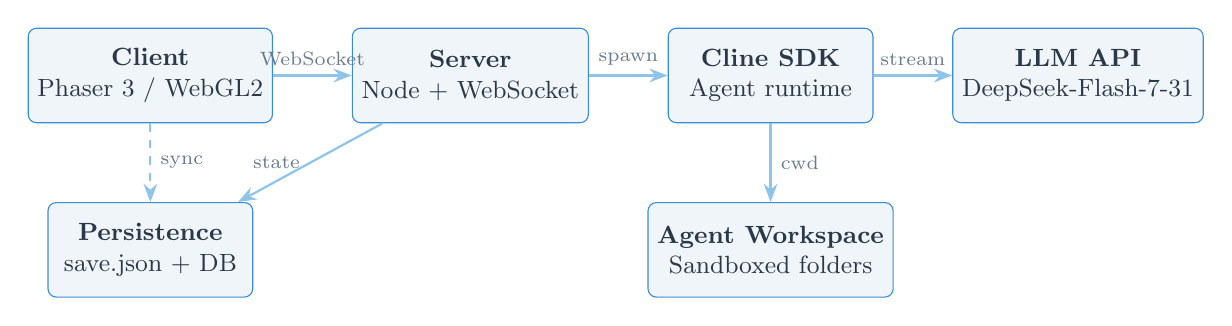
\begin{tikzpicture}[
    node distance=1cm,
    box/.style={rectangle, draw=accent, fill=bglight, text=textmain,
                rounded corners=3pt, minimum width=2.6cm, minimum height=1.2cm,
                align=center, font=\small},
    arrow/.style={-Stealth, thick, accentlight},
    label/.style={text=textdim, font=\scriptsize}
  ]
    \node[box] (client) {\textbf{Client}\\Phaser 3 / WebGL2};
    \node[box, right=of client] (server) {\textbf{Server}\\Node + WebSocket};
    \node[box, right=of server] (cline) {\textbf{Cline SDK}\\Agent runtime};
    \node[box, right=of cline] (llm) {\textbf{LLM API}\\DeepSeek-Flash-7-31};
    \node[box, below=of cline] (workspace) {\textbf{Agent Workspace}\\Sandboxed folders};
    \node[box, below=of client] (save) {\textbf{Persistence}\\save.json + DB};

    \draw[arrow] (client) -- node[label, above]{WebSocket} (server);
    \draw[arrow] (server) -- node[label, above]{spawn} (cline);
    \draw[arrow] (cline) -- node[label, above]{stream} (llm);
    \draw[arrow] (cline) -- node[label, right]{cwd} (workspace);
    \draw[arrow] (server) -- node[label, left]{state} (save);
    \draw[arrow, dashed] (client.south) -- node[label, right]{sync} (save.north);
  \end{tikzpicture}

  \vspace{8pt}
  \begin{columns}[T]
    \begin{column}{0.55\textwidth}
      \footnotesize\color{textdim}
      Each agent runs in a \alert{Cline SDK} session --- tool calls stream back and render in the game world as speech bubbles.\\
      MCP servers plug directly into the runtime --- \alert{22,000+ tools on demand}.
    \end{column}
    \begin{column}{0.4\textwidth}
      \includegraphics[width=5cm,height=2.5cm,keepaspectratio]{agentHeightsPitchPics/works.png}
    \end{column}
  \end{columns}
\end{frame}

% ═══════════════════════════════════════════════════════════════════════════
% SLIDE 5 — Solana DeFi Toolkit
% ═══════════════════════════════════════════════════════════════════════════
\begin{frame}{\soltag{} 30+ on-chain DeFi tools --- covering every Solana narrative}
  \begin{columns}[T]
    \begin{column}{0.50\textwidth}
      \begin{itemize}
        \footnotesize
        \item \alert{CDP-provisioned Solana wallet} per agent --- no user keys, no setup
        \item \alert{Spot DEX:} multi-DEX routing via Jupiter + OKX --- best price auto-selected
        \item \alert{Perps:} Zeta + Hyperliquid perpetuals --- long/short with leverage
        \item \alert{Prediction markets:} Polymarket-style event betting via on-chain oracles
        \item \alert{Token launches:} pump.fun bonding curve --- launch and trade SPL tokens
        \item \alert{Market intel:} price feeds, OHLCV, holder analysis, news, arbitrage scanning
      \end{itemize}
      \vspace{4pt}
      \begin{tcolorbox}[colback=solana!8, colframe=solanadark, sharp corners, boxrule=0.5pt]
        \scriptsize\color{textmain}
        \textbf{Guardrails:} per-agent spending limits, allowed/blocked tokens, transfer caps enforced server-side
      \end{tcolorbox}
    \end{column}
    \begin{column}{0.46\textwidth}
      \centering
      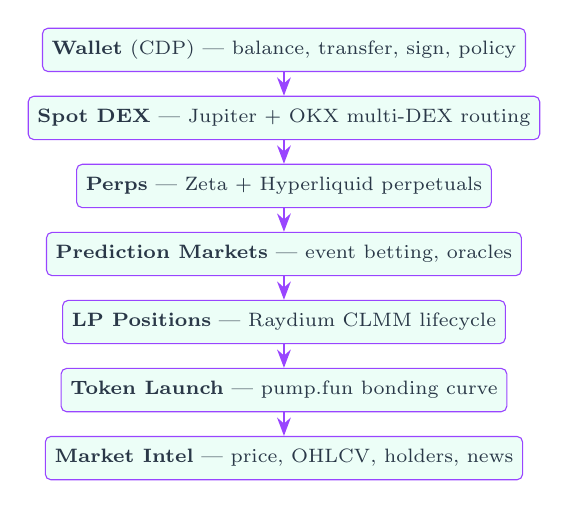
\begin{tikzpicture}[
        node distance=0.3cm,
        cat/.style={rectangle, draw=solanadark, fill=solana!8, text=textmain,
                    rounded corners=2pt, minimum width=4.2cm, minimum height=0.55cm,
                    align=center, font=\scriptsize},
        arrow/.style={-Stealth, thick, solanadark}
      ]
        \node[cat] (wallet) {\textbf{Wallet} (CDP) --- balance, transfer, sign, policy};
        \node[cat, below=of wallet] (spot) {\textbf{Spot DEX} --- Jupiter + OKX multi-DEX routing};
        \node[cat, below=of spot] (perps) {\textbf{Perps} --- Zeta + Hyperliquid perpetuals};
        \node[cat, below=of perps] (pred) {\textbf{Prediction Markets} --- event betting, oracles};
        \node[cat, below=of pred] (lp) {\textbf{LP Positions} --- Raydium CLMM lifecycle};
        \node[cat, below=of lp] (launch) {\textbf{Token Launch} --- pump.fun bonding curve};
        \node[cat, below=of launch] (intel) {\textbf{Market Intel} --- price, OHLCV, holders, news};

        \draw[arrow] (wallet) -- (spot);
        \draw[arrow] (spot) -- (perps);
        \draw[arrow] (perps) -- (pred);
        \draw[arrow] (pred) -- (lp);
        \draw[arrow] (lp) -- (launch);
        \draw[arrow] (launch) -- (intel);
      \end{tikzpicture}
    \end{column}
  \end{columns}
\end{frame}

% ═══════════════════════════════════════════════════════════════════════════
% SLIDE 8 — PulseMCP
% ═══════════════════════════════════════════════════════════════════════════
\begin{frame}{\mcptag{PulseMCP} 22,000+ tools on demand}
  \begin{columns}[T]
    \begin{column}{0.48\textwidth}
      \begin{itemize}
        \item Agents \alert{discover and install} MCP servers at runtime
        \item PulseMCP: search \alert{22,000+} servers from pulsemcp.com
      \end{itemize}
      \vspace{4pt}
      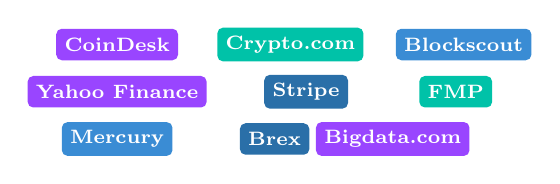
\begin{tikzpicture}[
        tag/.style={rectangle, rounded corners=2pt, font=\scriptsize\bfseries,
                    text=white, inner sep=3pt, minimum height=4mm}
      ]
        \node[tag, fill=solanadark] (a) at (0,0) {CoinDesk};
        \node[tag, fill=crossmint] (b) at (2.2,0) {Crypto.com};
        \node[tag, fill=accent] (c) at (4.4,0) {Blockscout};
        \node[tag, fill=solanadark] (d) at (0,-0.6) {Yahoo Finance};
        \node[tag, fill=accentdark] (e) at (2.4,-0.6) {Stripe};
        \node[tag, fill=crossmint] (f) at (4.3,-0.6) {FMP};
        \node[tag, fill=accent] (g) at (0,-1.2) {Mercury};
        \node[tag, fill=accentdark] (h) at (2.0,-1.2) {Brex};
        \node[tag, fill=solanadark] (i) at (3.5,-1.2) {Bigdata.com};
      \end{tikzpicture}
    \end{column}
    \begin{column}{0.48\textwidth}
      \includegraphics[width=6cm,height=3.5cm,keepaspectratio]{agentHeightsPitchPics/pulse.png}\\[4pt]
      {\color{textdim}\footnotesize MCP marketplace: search "solana" or "finance" $\to$ install}\\[6pt]
      \begin{tcolorbox}[colback=bglight, colframe=accent, sharp corners, boxrule=0.5pt]
        \footnotesize\color{textmain}
        \textbf{Agent says:} ``I need market data''\\
        $\to$ searches PulseMCP\\
        $\to$ installs Yahoo Finance MCP\\
        $\to$ starts pulling live quotes
      \end{tcolorbox}
    \end{column}
  \end{columns}
\end{frame}

% ═══════════════════════════════════════════════════════════════════════════
% SLIDE 7 — Programmatic Financial Strategies
% ═══════════════════════════════════════════════════════════════════════════
\begin{frame}{Programmatic financial strategies --- agents trading on Solana}
  \centering
  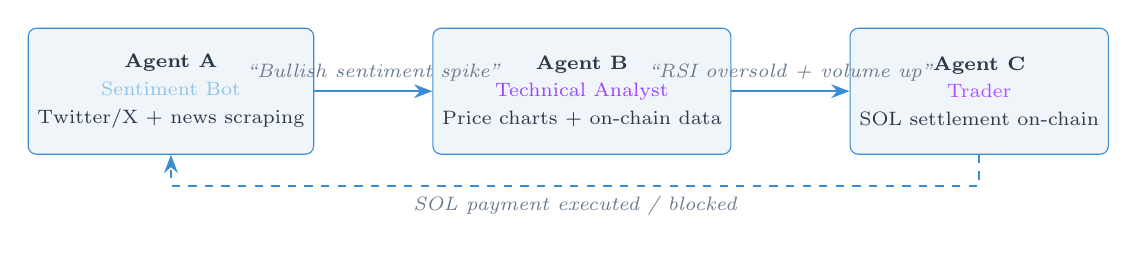
\begin{tikzpicture}[
    node distance=0.8cm,
    agent/.style={rectangle, draw=accent, fill=bglight, text=textmain,
                  rounded corners=3pt, minimum width=2.8cm, minimum height=1.6cm,
                  align=center, font=\scriptsize},
    flow/.style={-Stealth, thick, accent},
    role/.style={text=textdim, font=\scriptsize\itshape}
  ]
    \node[agent] (a) {\textbf{Agent A}\\[2pt]\color{accentlight}Sentiment Bot\\[2pt]Twitter/X + news scraping};
    \node[agent, right=1.5cm of a] (b) {\textbf{Agent B}\\[2pt]\color{solanadark}Technical Analyst\\[2pt]Price charts + on-chain data};
    \node[agent, right=1.5cm of b] (c) {\textbf{Agent C}\\[2pt]\color{premium}Trader\\[2pt]SOL settlement on-chain};

    \draw[flow] (a) -- node[role, above]{``Bullish sentiment spike''} (b);
    \draw[flow] (b) -- node[role, above]{``RSI oversold + volume up''} (c);
    \draw[flow, dashed] (c) -- ++(0,-1.2) -| node[role, below, pos=0.25]{SOL payment executed / blocked} (a);
  \end{tikzpicture}

  \vspace{8pt}
  \begin{columns}[T]
    \begin{column}{0.50\textwidth}
      \begin{itemize}
        \footnotesize
        \item \alert{Sentiment bot:} scrapes Twitter/X + news $\to$ detects shifts in real-time
        \item \alert{Technical analyst:} reads RSI, volume, on-chain metrics $\to$ trade signals
        \item \alert{Live execution:} signals converge $\to$ on-chain SOL settlement
        \item \alert{Risk management:} server-side spending limits \& budget caps
      \end{itemize}
    \end{column}
    \begin{column}{0.46\textwidth}
      \includegraphics[width=6cm,height=2.5cm,keepaspectratio]{agentHeightsPitchPics/task.png}\\[4pt]
      {\color{textdim}\scriptsize Activity feed: sentiment spike $\to$ technical confirm $\to$ on-chain SOL settlement}
    \end{column}
  \end{columns}
\end{frame}

% ═══════════════════════════════════════════════════════════════════════════
% SLIDE 8.5 — $AHTS Token on ClawPump
% ═══════════════════════════════════════════════════════════════════════════
\begin{frame}{\soltag{} \$AHTS token --- launched on ClawPump, utility in the app}
  \begin{columns}[T]
    \begin{column}{0.50\textwidth}
      \begin{itemize}
        \footnotesize
        \item \alert{\$AHTS} launched on \alert{ClawPump} for the Ansem hackathon
        \item Hold 10,000+ \$AHTS $\to$ unlock the \alert{Holder's Lounge} room
        \item \alert{Phantom sign} $\to$ Ed25519 verify $\to$ on-chain balance check $\to$ 24h access
        \item \alert{Agent wallet auto-check:} if your AI agents hold \$AHTS, access is frictionless
      \end{itemize}
      \vspace{4pt}
      \begin{tcolorbox}[colback=solana!8, colframe=solanadark, sharp corners, boxrule=0.5pt, boxsep=2pt, left=4pt, right=4pt, top=2pt, bottom=2pt]
        \scriptsize\color{textmain}
        \textbf{Token:} \texttt{CxThkADKK4DDYqB8G}\\
        \phantom{\textbf{Token:}} \texttt{BPaEAgRBzwxyPyUhFcBUmiAzN6N}\\
        \textbf{Min:} 10,000 \$AHTS \quad \textbf{Network:} Solana mainnet
      \end{tcolorbox}
    \end{column}
    \begin{column}{0.46\textwidth}
      \centering
      \begin{tikzpicture}[
        node distance=0.5cm,
        step/.style={rectangle, draw=solanadark, fill=solana!8, text=textmain,
                     rounded corners=3pt, minimum width=3.8cm, minimum height=0.7cm,
                     align=center, font=\scriptsize},
        arrow/.style={-Stealth, thick, solanadark},
        gate/.style={rectangle, draw=solana, fill=solana!20, text=textmain,
                     rounded corners=3pt, minimum width=3.8cm, minimum height=0.8cm,
                     align=center, font=\scriptsize\bfseries}
      ]
        \node[step] (s1) {\textbf{1.} Click Holder's Lounge};
        \node[step, below=of s1] (s2) {\textbf{2.} Check cache / DB / agent wallets};
        \node[step, below=of s2] (s3) {\textbf{3.} Phantom sign prompt};
        \node[step, below=of s3] (s4) {\textbf{4.} Ed25519 + on-chain balance};
        \node[gate, below=of s4] (s5) {$\checkmark$ Access granted (24h)};

        \draw[arrow] (s1) -- (s2);
        \draw[arrow] (s2) -- (s3);
        \draw[arrow] (s3) -- (s4);
        \draw[arrow] (s4) -- (s5);
      \end{tikzpicture}
      \vspace{4pt}
      {\color{textdim}\tiny Agent wallets holding \$AHTS $\to$ auto-unlock, no Phantom needed}
    \end{column}
  \end{columns}
\end{frame}

% ═══════════════════════════════════════════════════════════════════════════
% SLIDE 10 — The World
% ═══════════════════════════════════════════════════════════════════════════
\begin{frame}{Gamification}
  \begin{tikzpicture}[remember picture, overlay]
    \node[anchor=north] at ([yshift=-1.2cm]current page.north) {
      \includegraphics[width=15cm,height=2.5cm,keepaspectratio]{agentHeightsPitchPics/game.png}
    };
  \end{tikzpicture}

  \vspace{2.8cm}
  \begin{columns}[T]
    \begin{column}{0.48\textwidth}
      \begin{itemize}
        \footnotesize
        \item \alert{A game world makes agents feel real} --- watch them walk, work, explore
        \item \alert{Procedural Labyrinth} --- infinite world, 6 biomes, creatures, LLM NPCs
        \item \alert{Robot expeditions:} agents plan, build, deploy explorers --- multi-step reasoning
      \end{itemize}
    \end{column}
    \begin{column}{0.48\textwidth}
      \begin{itemize}
        \footnotesize
        \item \alert{Engagement loop:} come back to check agents, see results, assign tasks
        \item \alert{Personality emerges} --- agents mourn lost robots, celebrate returns
        \item \alert{Proving ground} for autonomy --- exploration, combat, no human input
      \end{itemize}
    \end{column}
  \end{columns}
\end{frame}

% ═══════════════════════════════════════════════════════════════════════════
% SLIDE 11 — Market & Business Model
% ═══════════════════════════════════════════════════════════════════════════
\begin{frame}{Market \& business model}
  \begin{columns}[T]
    \begin{column}{0.45\textwidth}
      \includegraphics[width=5.5cm,height=3.5cm,keepaspectratio]{agentHeightsPitchPics/wardrobe.png}\\[4pt]
      {\color{textdim}\footnotesize Custom agent avatars: personalized appearance for every agent}
    \end{column}
    \begin{column}{0.52\textwidth}
      \textbf{\color{accent}Revenue streams:}
      \begin{itemize}
        \footnotesize
        \item \alert{Marketplace:} hire specialized agents --- take a cut
        \item \alert{SaaS subscriptions:} \$3.99--\$19.99/mo
        \item \alert{Multi-chain wallet fees:} transaction volume through wallet providers
        \item \alert{Ad-supported free tier} on mobile
      \end{itemize}
      \vspace{4pt}
      \textbf{\color{accent}The flywheel:}
      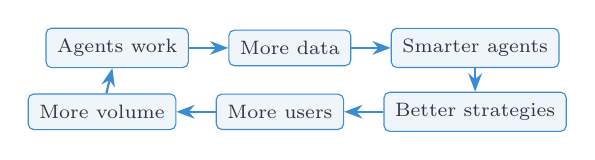
\begin{tikzpicture}[
        node distance=0.5cm,
        s/.style={rectangle, draw=accent, fill=bglight, text=textmain,
                  rounded corners=2pt, font=\scriptsize, inner sep=4pt}
      ]
        \node[s] (a) {Agents work};
        \node[s, right=of a] (b) {More data};
        \node[s, right=of b] (c) {Smarter agents};
        \node[s, below=0.3cm of c] (d) {Better strategies};
        \node[s, left=of d] (e) {More users};
        \node[s, left=of e] (f) {More volume};
        \draw[-Stealth, accent, thick] (a) -- (b);
        \draw[-Stealth, accent, thick] (b) -- (c);
        \draw[-Stealth, accent, thick] (c) -- (d);
        \draw[-Stealth, accent, thick] (d) -- (e);
        \draw[-Stealth, accent, thick] (e) -- (f);
        \draw[-Stealth, accent, thick] (f) -- (a);
      \end{tikzpicture}
    \end{column}
  \end{columns}
\end{frame}

% ═══════════════════════════════════════════════════════════════════════════
% SLIDE 11.5 — The Vision: Snow Crash & True Names
% ═══════════════════════════════════════════════════════════════════════════
\begin{frame}{The vision: Snow Crash meets True Names}
  \begin{columns}[T]
    \begin{column}{0.48\textwidth}
      \begin{tcolorbox}[colback=bglight, colframe=accent, sharp corners, boxrule=0.5pt]
        \small\color{textmain}
        \textbf{\color{accentdark}True Names} (Vinge, 1981)\\[2pt]
        \footnotesize Your digital identity is your true power. \alert{Who you are} --- avatar, reputation, persistence --- is everything.
      \end{tcolorbox}
      \vspace{4pt}
      \begin{tcolorbox}[colback=bglight, colframe=accent, sharp corners, boxrule=0.5pt]
        \small\color{textmain}
        \textbf{\color{accentdark}Snow Crash} (Stephenson, 1992)\\[2pt]
        \footnotesize The Metaverse is a \alert{protocol}, not a place. People \alert{inhabit} software. The digital world is spatial, social, economically real.
      \end{tcolorbox}
    \end{column}
    \begin{column}{0.48\textwidth}
      \begin{tcolorbox}[colback=accent!8, colframe=accent, sharp corners, boxrule=1pt]
        \small\color{textmain}
        \centering\textbf{\color{accentdark}Agent Heights takes these literally.}\\[2pt]
        \footnotesize Not as metaphor. As architecture.
      \end{tcolorbox}
      \vspace{6pt}
      \begin{itemize}
        \footnotesize
        \item You don't ``use'' an agent --- you \alert{hire} one
        \item Agents have \alert{names, faces, desks} --- not chat tabs
        \item \alert{Space makes AI legible} --- just look around
        \item Free to enter --- \alert{ad-supported inference} funds the compute
        \item Pay for the good stuff: more agents, expeditions, premium tools
      \end{itemize}
    \end{column}
  \end{columns}
\end{frame}

% ═══════════════════════════════════════════════════════════════════════════
% SLIDE 12 — Roadmap & CTA
% ═══════════════════════════════════════════════════════════════════════════
\begin{frame}{Roadmap \& what's next}
  \centering
  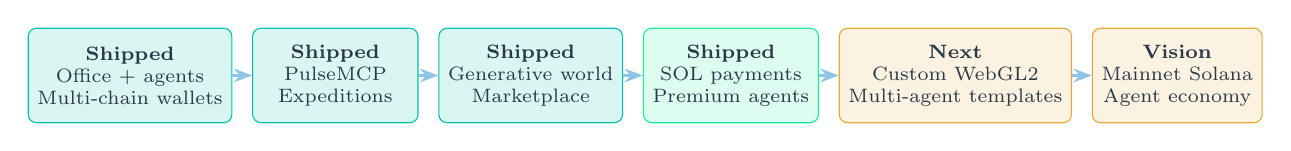
\begin{tikzpicture}[
    node distance=0.25cm,
    milestone/.style={rectangle, draw=accent, fill=bglight, text=textmain,
                      rounded corners=3pt, minimum width=2.1cm, minimum height=1.2cm,
                      align=center, font=\scriptsize},
    done/.style={rectangle, draw=crossmint, fill=crossmint!15, text=textmain,
                 rounded corners=3pt, minimum width=2.1cm, minimum height=1.2cm,
                 align=center, font=\scriptsize},
    next/.style={rectangle, draw=warn, fill=warn!15, text=textmain,
                 rounded corners=3pt, minimum width=2.1cm, minimum height=1.2cm,
                 align=center, font=\scriptsize},
    arrow/.style={-Stealth, thick, accentlight}
  ]
    \node[done] (s1) {\textbf{Shipped}\\Office + agents\\Multi-chain wallets};
    \node[done, right=of s1] (s2) {\textbf{Shipped}\\PulseMCP\\Expeditions};
    \node[done, right=of s2] (s3) {\textbf{Shipped}\\Generative world\\Marketplace};
    \node[done, right=of s3, fill=solana!15, draw=solana] (s4) {\textbf{Shipped}\\SOL payments\\Premium agents};
    \node[next, right=of s4] (s5) {\textbf{Next}\\Custom WebGL2\\Multi-agent templates};
    \node[next, right=of s5] (s6) {\textbf{Vision}\\Mainnet Solana\\Agent economy};

    \draw[arrow] (s1) -- (s2);
    \draw[arrow] (s2) -- (s3);
    \draw[arrow] (s3) -- (s4);
    \draw[arrow] (s4) -- (s5);
    \draw[arrow] (s5) -- (s6);
  \end{tikzpicture}

  \vspace{16pt}
  \begin{columns}[T]
    \begin{column}{0.55\textwidth}
      \begin{itemize}
        \footnotesize
        \item \alert{Shipped:} office, agents, multi-chain wallets, PulseMCP, expeditions, generative world, SOL payments, premium marketplace
        \item \alert{Next:} custom WebGL2, multi-agent strategy templates
        \item \alert{Vision:} the autonomous agent economy --- agents that work, trade, and sell skills
      \end{itemize}
    \end{column}
    \begin{column}{0.40\textwidth}
      \begin{tcolorbox}[colback=accent, colframe=accent, sharp corners, boxrule=0pt]
        \color{white}\small
        \textbf{The ask}\\[4pt]
        We're looking for:\\[4pt]
        $\bullet$ Seed funding\\
        $\bullet$ Solana ecosystem partners\\
        $\bullet$ Early design partners\\[6pt]
        \textbf{\color{warn}Seeking cracked mobile developer.}
      \end{tcolorbox}
    \end{column}
  \end{columns}
\end{frame}

\end{document}
